 \documentclass[10pt,landscape, margin = 0.1mm]{article}
\usepackage{amssymb,amsmath,amsthm,amsfonts}
\usepackage{multicol,multirow}
\usepackage{graphicx}
\usepackage{float}
\usepackage{graphicx}
\usepackage{subcaption}
\usepackage{calc}
\usepackage[dvipsnames]{xcolor}
\usepackage{ifthen}
\usepackage{titlesec}
\usepackage[landscape]{geometry}
\usepackage{enumitem}
\usepackage{syntonly}
\usepackage[most]{tcolorbox}
\setitemize{noitemsep,topsep=0pt,parsep=0pt,partopsep=0pt}
\usepackage[colorlinks=true,citecolor=blue,linkcolor=blue]{hyperref}
\usepackage{tikz}
\usepackage{stmaryrd}
\usepackage{listings}
\usepackage{booktabs}
\usepackage{xcolor}
\usepackage{bussproofs}
\def\proofSkipAmount{\vskip -10pt}
\usepackage{stmaryrd}


\def\cm{\tikz\fill[scale=0.4](0,.35) -- (.25,0) -- (1,.7) -- (.25,.15) -- cycle;} 
\ifthenelse{\lengthtest { \paperwidth = 11in}}
    { \geometry{top=.1in,left=.1in,right=.1in,bottom=.1in} }
	{\ifthenelse{ \lengthtest{ \paperwidth = 297mm}}
		{\geometry{top=1mm,left=1mm,right=1mm,bottom=1mm} }
		{\geometry{top=1mm,left=1mm,right=1mm,bottom=1mm} }
	}

\pagestyle{empty}

\makeatletter

 

\newcommand{\nextcol}{\vfill\null\columnbreak}


\titleformat{\subsection}
  {\normalfont\fontsize{10}{10}\bfseries}{\thesection}{1em}{}

\newcommand*{\mysection}[2][black]{\vskip 0pt \vspace{2pt}\section{#2}\vspace{2pt} \colorlet{chaptercolor}{#1}}


\newcommand*{\mysubsection}[1]{\vspace{-3mm}

\color{chaptercolor}\subsection{ #1 }
\vspace{0.4mm}\color{black}
\vspace{-2mm}}

\tcbset {
  base/.style={
    arc=0mm, 
    bottomtitle=0.5mm,
    boxrule=0mm,
    colbacktitle=black!10!white, 
    coltitle=black, 
    fonttitle=\bfseries, 
    left=2.5mm,
    leftrule=1mm,
    right=3.5mm,
    title={#1},
    toptitle=0.75mm, 
  }
}

\newtcolorbox{mainbox}[2]{
  breakable,
  colframe={#2}, 
  base={#1} 
}

\definecolor{cadet}{rgb}{0.37, 0.62, 0.63}
\definecolor{MutedCoral}{rgb}{0.87, 0.49, 0.42}  
\definecolor{SoftMustard}{rgb}{0.85, 0.76, 0.42} 
\definecolor{PaleSage}{rgb}{0.68, 0.81, 0.68}   
\definecolor{DustyLavender}{rgb}{0.69, 0.60, 0.85} 
\definecolor{col1}{rgb}{0.0, 0.0, 1.0}    % Blue
\definecolor{col2}{rgb}{0.0, 0.5, 0.75}   % Light Blue
\definecolor{col3}{rgb}{0.0, 0.75, 0.5}   % Light Greenish Blue
\definecolor{col4}{rgb}{0.0, 1.0, 0.25}   % Light Green
\definecolor{col5}{rgb}{0.0, 1.0, 0.0}    % Green

\newcommand{\BDEF}[2]{\begin{mainbox}{#1}{cadet} 
    #2
\end{mainbox}}

\newcommand{\BCODE}[2]{\begin{mainbox}{#1}{PaleSage} 
    #2
\end{mainbox}}

\newcommand{\BEX}[2]{\begin{mainbox}{#1}{DustyLavender} 
    #2
\end{mainbox}}


\newcommand{\BRE}[2]{\begin{mainbox}{#1}{SoftMustard} 
    #2
\end{mainbox}}

\newcommand{\COM}[1]{}
\definecolor{matplotlibgreen}{rgb}{0.0, 0.3804, 0.0}
\definecolor{matplotlibred}{rgb}{0.8588, 0.0, 0.0}

\makeatother
\setcounter{secnumdepth}{0}
\setlength{\parindent}{0pt}
\setlength{\parskip}{0pt plus 0.5ex}
\setlength{\marginparwidth}{0pt}
\setlength{\marginparsep}{0pt}

\lstset{
  language=OCaml,
  basicstyle=\ttfamily\scriptsize,
  columns=fullflexible,
  showstringspaces=false
}

\begin{document}

\syntaxonlys

\begin{center}
     \Large{\textbf{Cheat Sheet}: Comp Sc BSc, CompDes - Surname Name, DD.MM.YYYY - \textbf{XX-YYY-ZZZ}} \\
\end{center}
\begin{multicols}{3}
\setlength{\premulticols}{0.5pt}
\setlength{\postmulticols}{0.5pt}
\setlength{\multicolsep}{0.5pt}
\setlength{\columnsep}{0.2pt}
\setlength{\columnseprule}{0pt}



\begin{flushleft}

\mysection[black]{1. OCAML}


\begin{itemize} [leftmargin = *,noitemsep]
    \item  F' are right-associative: $t_{1} \rightarrow t_{2}  \rightarrow t_3 \equiv  t_1  \rightarrow (t_2  \rightarrow t_3)$
    \item F' application is left-associative: $f\,x\,y \equiv (fx)y$
\end{itemize}
\begin{multicols}{2}
\textbf{Head-Recursive}
\begin{lstlisting}
let rec sum xs =
  match xs with
  | [] -> 0
  | x :: xs' -> x + sum xs'
\end{lstlisting}
\columnbreak
\textbf{Tail-Recursive}
\begin{lstlisting}
let sum xs =
  let rec aux acc xs =
    match xs with
    | [] -> acc
    | x :: xs' -> aux (acc + x) xs'
  in
  aux 0 xs
\end{lstlisting}
\end{multicols}











\mysection[black]{2. x86lite and LLVM}

\mysubsection{2.1 x86lite}




\BDEF{Calling Convention}{
\textbf{Args 1-6} in \texttt{rdi rsi rdx rcx r8 r9}; args $\ge7$ on stack (pushq in rev. order);
\textbf{return} in \texttt{rax};
\textbf{caller-saves} \texttt{rax rcx rdx rsi rdi r8-r11};
\textbf{callee-saves} \texttt{rbx rbp (top) r12-r15}
}
\textbf{Instr.}: INSTR SRC DEST, reg. with \%, imm. with \$, $(A)$ mem. at the address stored in $A$ \\
\textbf{Sfx.}:b=1,l=2,w=4,q=8 bytes\\
\textbf{Args.}: for $n\ge 7:\text{addr}=((n-7)+2)\cdot 8 + \%\text{rbp}$
\begin{multicols}{4}
\textbf{Prologue}
\begin{lstlisting}
 pushq %rbp
 movq %rsp,%rbp
 subq $x,%rsp
\end{lstlisting}
\columnbreak
\textbf{Epilogue}
\begin{lstlisting}
 addq $x,%rsp
 popq %rbp
 retq
\end{lstlisting}
\columnbreak
\textbf{Push}\\
\begin{lstlisting}
pushq %X:
 rsp <- rsp-8
 Mem[rsp] <- X
\end{lstlisting}
\columnbreak
\textbf{Pop}\\
\begin{lstlisting}
popq %X:
 X <- Mem[rsp]
 rsp <- rsp+8 
\end{lstlisting}
\end{multicols}
\textbf{Flg}: OF = under-/overflow, SF = sign (1=neg.),ZF=0
\textbf{CC}: $e=\text{ZF}$,$ne=\neg\text{ZF}$, $g=\neg \text{ZF}\wedge \text{SF}{=}\text{OF}$,$l=\text{SF}\neq \text{OF}$,$ge=\text{SF}=\text{OF}$,$le=\text{ZF}\vee\text{SF} \neq \text{OF}$
\textbf{CC (Signed) x86}: \texttt{cmpq SRC, DST} then: \texttt{je / jz (DST == SRC),jne / jnz (DST != SRC),jl[e] (DST <[=]  SRC),jg[e] (DST >[=]  SRC)}
\textbf{Unsigned}: \texttt{je/jz (DST == SRC),jne/jnz (DST != SRC),jb[e] (DST <[=] SRC),ja[e] (DST >[=] SRC)}\\
\textbf{LLVM}: 
\texttt{\%c = icmp sgt i64 \%a \%b}. \texttt{\#c} is 1 iff \texttt{\%a<\%b}. More: \texttt{eq, ne, sgt, sge, slt, sle} 


\mysubsection{2.2 LLVM}
\textbf{Prefix}: local (\texttt{\%}) / global (\texttt{@}) identifier\\
\textbf{Phi-Nodes}: \lstinline[language=llvm]{%val = phi <ty> [%v1, %l1], [%v2, %l2]}
, select based most recent block visited\\ 
\textbf{GEP}:  \lstinline[language=llvm]{<res> = getelementptr <ty>, <ty>* <ptr>, <idxs>...},
purely arithmetic, if nested pointers \lstinline[language=llvm]{GEP(load(GEP(p*)))} \\


\textbf{Alloca \& Stack Storage:}  Allocates stack space, returns pointer, is freed on function return.

\textbf{Memory}: $8$(long), $4$(int) $\cdot \# $ vars. needed after func. call.
\begin{tabular}{@{}l l l@{}}
\toprule
\textbf{LLVM} & \textbf{x86 Equivalent} \\
\midrule
\texttt{sub i64 O1, O2} \textcolor{gray}{= o1 - o2} & \texttt{sub1 SRC, DST} \textcolor{gray}{= dst - src} \\
\texttt{\%L = alloca <ty>}  & \texttt{subq sizeof(T), \%rsp} \\
\texttt{\%L = load <ty>* P} & \texttt{movq (SRC), DST} \\
\texttt{store <ty> V, <ty>* P}  & \texttt{movq SRC, (DST)} \\
\midrule
\texttt{call <ty> F(...)} & \texttt{callq F} \\
\texttt{ret void / <ty>}  & \texttt{retq} \\
\texttt{br label \%L} & \texttt{jmp \%L} \\
\texttt{br i1 C, \%L1, \%L2} & \texttt{jne \%L1; jmp \%L2} \\
\midrule
\texttt{icmp <cond> ...} & \texttt{cmpq} + \texttt{jcc} \\
\texttt{getelementptr} & \texttt{leaq} (often) \\
\bottomrule
\end{tabular}







\mysection[black]{3. Lexing and Parsing}


\mysubsection{3.1 Lexing}
\BDEF{Regular Expresssions}{
Define  sets of strings precisely
\begin{tabular}{@{}l l l l@{}}
\toprule
\textbf{Expr.} & \textbf{Desc.} & \textbf{Expr.} & \textbf{Equiv.} \\
\midrule

$\epsilon$ 
& empty 
& $R?$ 
& $(\epsilon \mid R)$ \\

 \texttt{'a'} 
& char 
& \texttt{"foo"} 
& \texttt{'f''o''o'} \\

$R_1 \mid R_2$ 
& $R_1$ or $R_2$ 
& $R^+$ 
& $RR^*$ \\

$R_1 R_2$ 
& $R_2$ follows $R_1$ 
& \texttt{['a'-'z']} 
& $(a \mid \dots \mid z)$ \\

$R^*$ 
& $0 \leq$ reps. 
& \texttt{[\^\,'0'-'9']} 
&  $\mathbf{C}$\texttt{['a'-'z']}  \\
\end{tabular}} 
\textbf{Lexer Generator}: Associate $R_i$ with action $A_i$\\
\textbf{NFA to DFA}: Powerset; collapses $\epsilon$-transitions
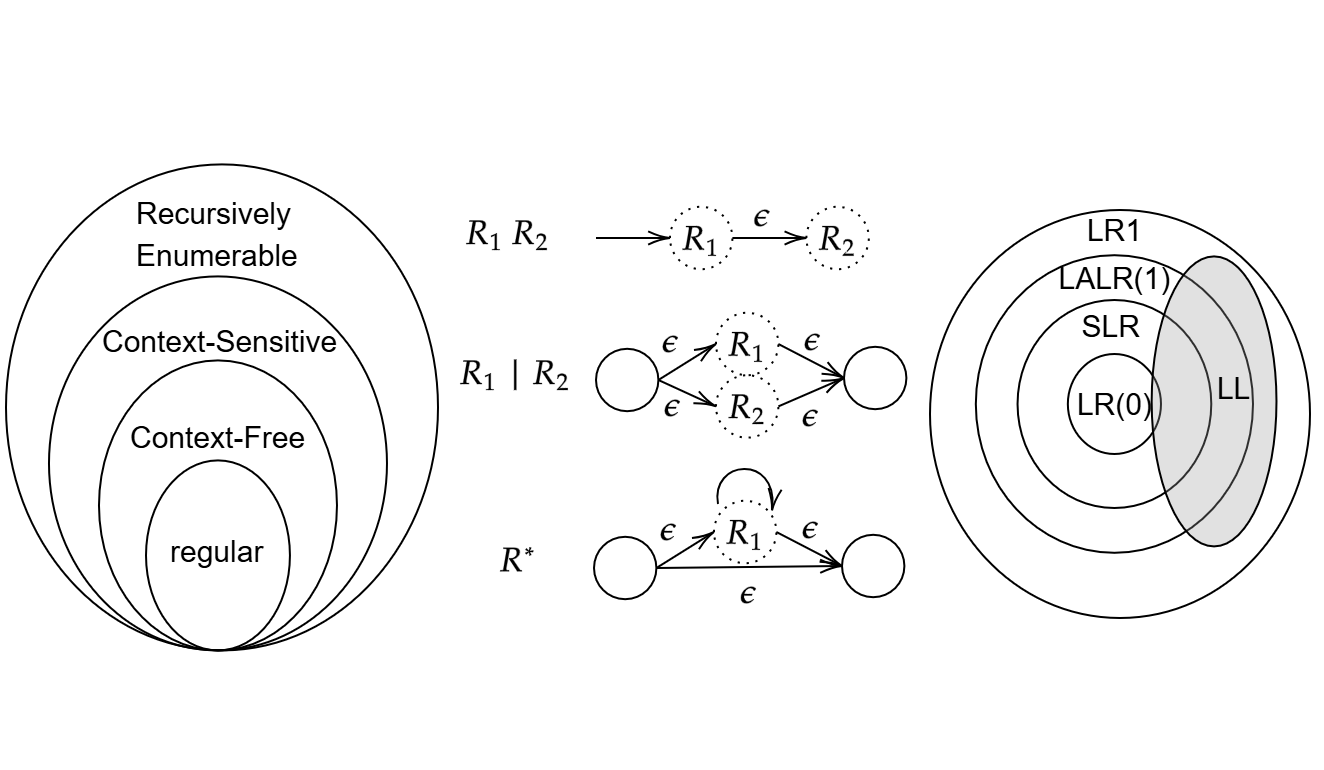
\includegraphics[width=1\linewidth]{images/diagram-lexing-parsing.png}


\mysubsection{3.2 Parsing}
\textbf{Context-Free Grammars (CFG)}: consists of: \textcolor{Aquamarine}{tree-rep}
\begin{itemize}[leftmargin = *,noitemsep]
\item \textbf{Terminals:} lexical token, $\alpha, \beta, (,),..$ ($\epsilon$ isn't) \textcolor{Aquamarine}{leaves}
\item \textbf{NonTerm.:} Syntactic var. $S,T,S',...$ \textcolor{Aquamarine}{internal nodes}
\item \textbf{Production:} Rule $T \mapsto \beta$, which gives $\alpha T \gamma \mapsto \alpha \beta \gamma$
\item \textbf{Start Symbol:} Nonterminal 
 \end{itemize}
 \textbf{LL(k)/LR(k)}: Left-to-right scanning, Right-/Leftmost deriv., k lookahead\\
\textbf{Empty Lang.}: $\not \exists$ finite derivation\\
\textbf{Productiveness}: Rule contains terminal\\
\textbf{Parse-Trees}: Left-/Rightmost derivation yields same tree, order of application not contained\\
\begin{multicols}{2}
\textbf{Left-recursive}\\
$E \mapsto ET$\\ 
LL(1)-incompatible  ($\infty$-rec)\\
LR(1)-compatible

\columnbreak

\textbf{Right-recursive}\\
$E \mapsto TE$\\ 
LL(1)-compatible\\
LR(1)-compatible

\end{multicols}
\textbf{Ambiguity}: Remove my allowing only left-/right-recursion, adding non-terminals\\
\textbf{Precendence}: Determined by how deep (far from the start symbol) an operator is introduced in the grammar. {\color{Aquamarine}$S \to S+S\mid S*S\mid num$ to $S\to T * S \mid T$,$T\to N + T \mid N$,$N\to num $, prec: $+>*$ }\\
\textbf{Mult. Derivations}: An unambiguous CFG can have more than one derivation, all of them correspond to the same abstract syntax tree\\
\textbf{Converting to LL(1)}: $A \mapsto \alpha \beta_1 \mid \alpha \beta_2$ to $A \mapsto \alpha A'$, $A' \mapsto \beta_1$,$A' \mapsto \beta_2$\\



\textbf{Remove Left-Rec./Enforce Right Assoc.}: $A \mapsto A\alpha_1 \mid \ldots  \mid A \alpha_n \mid \beta_1 \mid \ldots \mid \beta_m$ to $A \mapsto \beta_1 A' \mid \ldots  \mid \beta_m A'$, $A' \mapsto \alpha_1 A' \mid \ldots \mid \alpha_n A' \mid \epsilon$ {\color{Aquamarine}$S \to S+S\mid S*S\mid n$ to $S\to n S'$,$S'\to+SS'\mid *SS'\mid \epsilon$} \\




\textbf{Predictive Parsing (PP)}: Given LL(1), lookahead symbol uniquely defines production to apply.\\
\textbf{PP Table}: $\operatorname{nonterminal}\times \operatorname{lookahead} \mapsto \operatorname{production}$\\
\textbf{First}: Pot. start. char $\operatorname{Fst}(\alpha A)=\{\alpha\}$,$\operatorname{Fst}(A\alpha)=\operatorname{Fst}(A)$\\
\textbf{Follow}: terminals that may follow $\$\in \operatorname{Fl}(S)$, $A\mapsto \alpha B a \beta\Rightarrow a \in \operatorname{Fl}(B)$,$A\mapsto \alpha B C \beta \Rightarrow \operatorname{Fst}(C)\setminus \epsilon \subseteq \operatorname{Fl}(B)$. $A\mapsto \alpha B \beta \wedge \epsilon \in \operatorname{Fst}(\beta) \Rightarrow \operatorname{Fl}(A) \subseteq \operatorname{Fl}(B) $ \\
\textbf{Top-down (TD)/Bottom-Up (BU)}: Direction of building parse tree, LL = TD- / LR =BU-parsers \\
\textbf{Shift-Reduce Parser (SRP)}: Algo to impl. LR-pars., $\forall$ LR-parsers are SRP, uses:
\begin{itemize}[leftmargin = *,noitemsep]
\item \textbf{Shift:} Move look-ahead token to stack
\item \textbf{Reduce:} Replace symbols on top of stack with non-terminals
 \end{itemize}
 \textbf{Ex:} Given $S \mapsto S + E \mid E$(1) ,$E \mapsto \operatorname{number}$ (2)
\begin{multicols}{3}
\textbf{Stack}\\
- \\
\texttt{1} \\
\texttt{E} \\
\texttt{S} \\

\columnbreak
\textbf{Input}\\
\texttt{1 + 2} \\
\texttt{ + 2} \\
\texttt{ + 2} \\
\texttt{ + 2}\\
\columnbreak
\textbf{Action}\\
shift \texttt{1} \\
reduce (2) \\
reduce (1) \\
shift  \texttt{+}


\end{multicols}

\textbf{LR(0)}: No look-ahead, state given by $A\mapsto \alpha.\beta$, $\alpha$ consumed, $\beta$ potential upcoming input, tracks corrent state, if $\beta = \epsilon$, eligible for reduction\\
\textbf{Action Selection Problem}: Both shift and reduce may be possible, not clear what to take\\
\textbf{LR(0) to DFA}:   \textcolor{Aquamarine}{Example} ${\color{Aquamarine}S\mapsto (L) \mid id, L\to S \mid L,S}$
\begin{enumerate}[leftmargin = *,noitemsep]
\item Add $S' \mapsto S\$$ to grammar
\item Add Initial item with empty lookahead ${\color{Aquamarine}S'\mapsto .S \$, \{\}}$
\item If state contains dot before nonterminal, compute closure of state with lookahead ${\color{Aquamarine}S'\mapsto .S \$,S\mapsto . (L),\{\$\};S\mapsto . \operatorname{id},\{\$\}}$   
\item Add transition for each non-/terminal after the dot.  , the new state moves the dot  \textcolor{Aquamarine}{Transitions: ${\color{Aquamarine}\operatorname{id},(,S}$}, \textcolor{Aquamarine}{Added States: ${\color{Aquamarine}S'\mapsto S. \$,S\mapsto (.L),S\mapsto  \operatorname{id}.}$   }
\item For each new state start with step 3. again
\end{enumerate}


\textbf{Parsing-Table (LR0)}: Possible actions, use to determine parsing
$$( s, X) \mapsto
\begin{cases}
\text{shift } + \text{goto } s' & X \in \operatorname{terminal} \\
\text{goto } s' & X \in \operatorname{non-terminal} \\
\text{reduce } A \to \alpha
\end{cases}
$$
\textbf{Limitations}: Only works if reduce actions are unique, otherwise shift/reduce or reduce/reduce conflicts\\
\textbf{LR(1)}: Item is LR(0) item with look-ahead\\
\textbf{LR(1) closure}: \\$\forall [A \rightarrow \alpha \cdot B \beta, t] \text{ in } S;\forall \text{production } B \rightarrow \gamma \text{ in } G;
\forall \text{ token } b \text{ in } \text{FIRST}(\beta t); \text{Add } [B \rightarrow \cdot \gamma, b] \text{ to } S$\\


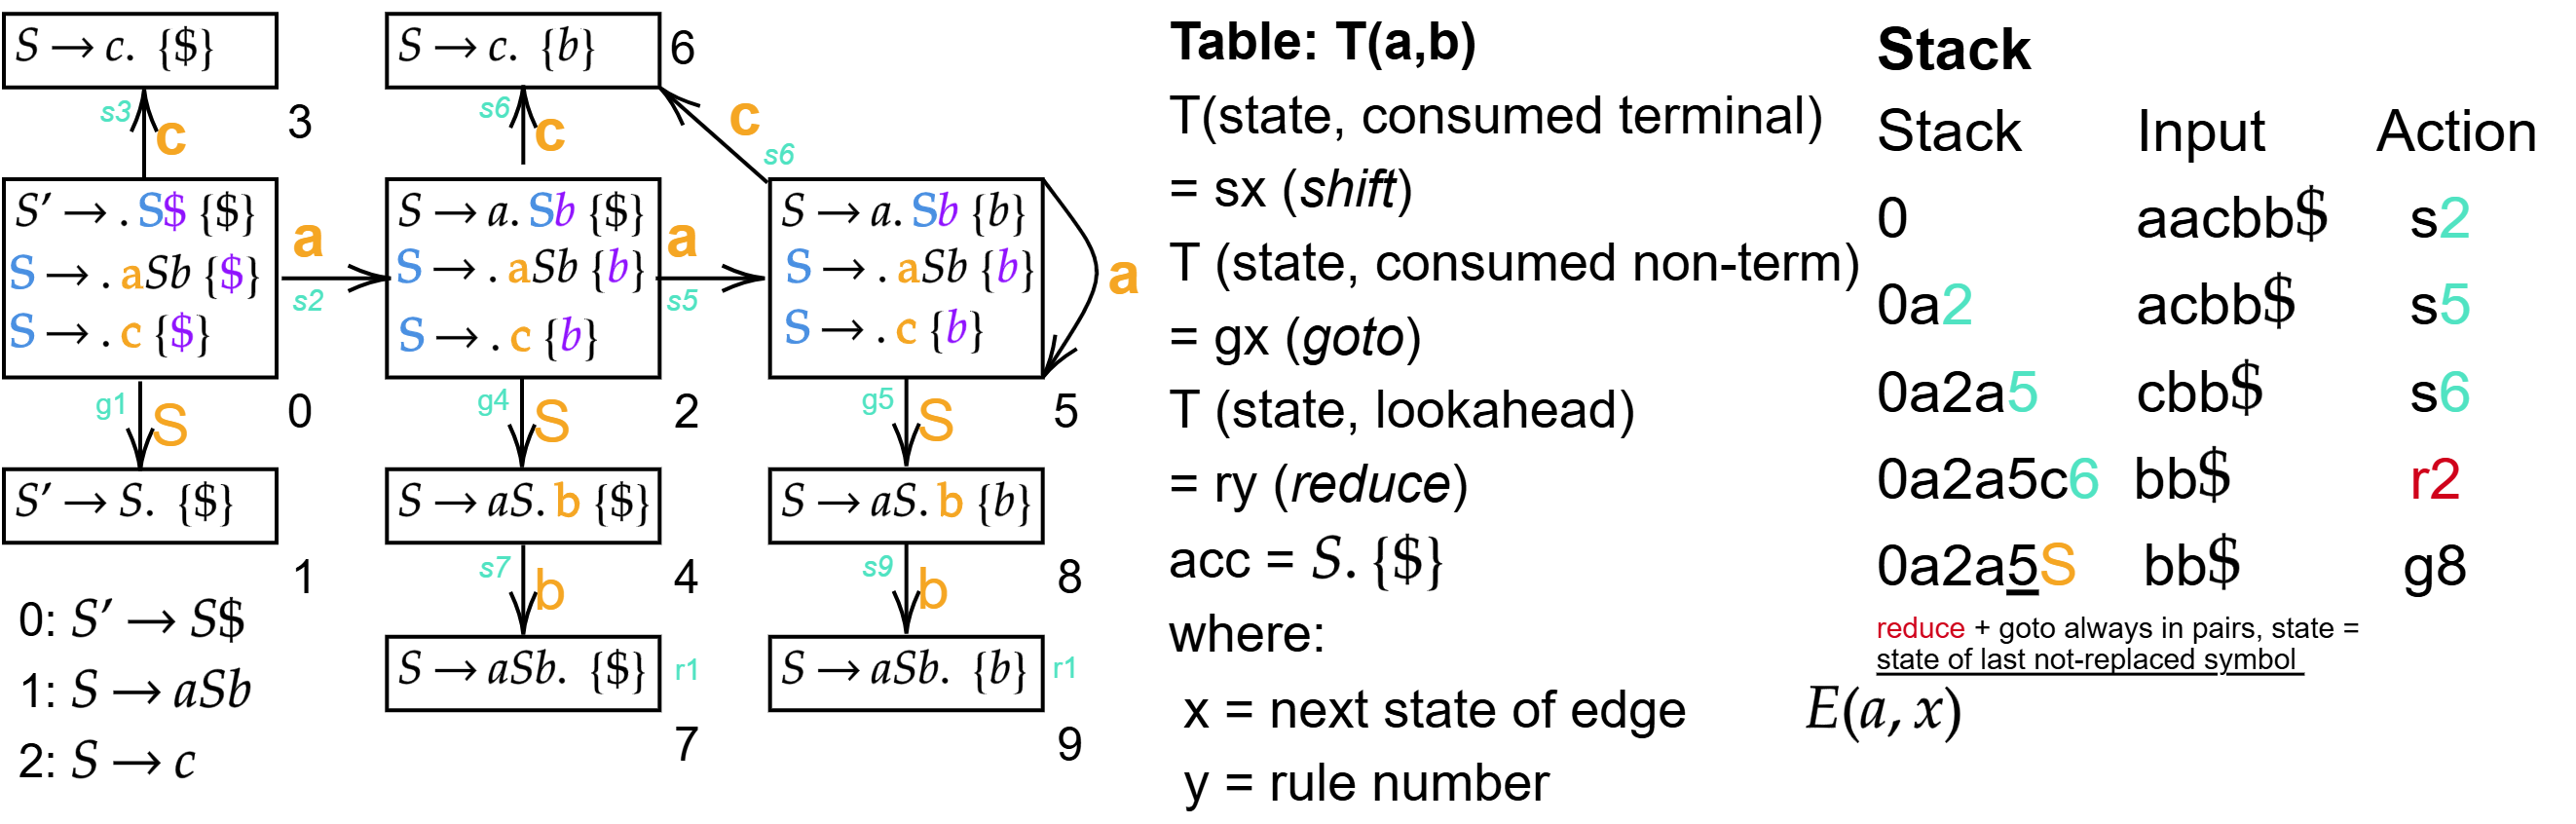
\includegraphics[width=1\linewidth]{images/parsing-table.png}


\textbf{LALR(1)}: Merging LR(1) states that have the same LR(0) core and combine look-ahead, factor 10 fewer states, may only introduce reduce/reduce conflicts i.e. $[X \mapsto a. , a],[X \mapsto a. , b] \Rightarrow [X \mapsto a. , a/b]$\\
\textbf{SLR}: Simple LR, uses follow     \\
\textbf{GLF}: Generalized LR, computes all parses for input and disambiguate based on context \\



\mysection[black]{4. Types}



\mysubsection{4.1 Lambda Calculus}
\textbf{Lambda Calculus}: \texttt{(fun x -> e)}, or $\lambda x.e$, turing complete 

 \begin{multicols}{2}
\textbf{Abstract Syntax}\\
\begin{lstlisting}
type exp =
| Var of var
| Fun of var * exp 
| App of exp * exp
\end{lstlisting}
\columnbreak

\textbf{Concrete Syntax}\\
\begin{lstlisting}
exp ::=
| x 
| fun x -> exp 
| exp1 exp2 
| ( exp )
\end{lstlisting}
\end{multicols}
\textbf{Application}: Interpreted by substitution {\scriptsize\texttt{(fun x -> fun y -> x + y) 1= subst 1 x (fun y -> x + y)= (fun y -> 1 + y)}}
\textbf{Substitute}: free $x$ with $y$ in $e$: \texttt{e\{y/x\}}, cases:
\begin{itemize}[leftmargin = *,noitemsep]

\item \textbf{Variable (matching):}  
\texttt{x\{v/x\} = v}.

\item \textbf{Variable (non-matching):}  
\texttt{y\{v/x\} = y} if $x \neq y$.

\item \textbf{Function (shadowing):}  
\texttt{(fun x -> exp)\{v/x\} = fun x -> exp}.

\item \textbf{Function (non-shadowing):}  
\texttt{(fun y -> exp)\{v/x\} = fun y -> exp\{v/x\}} if $x \neq y$.

\item \textbf{Application:}  
\texttt{(e$_1$ e$_2$)\{v/x\} = (e$_1$\{v/x\} e$_2$\{v/x\})}.
\end{itemize}

\textbf{Free/Bound:} In \texttt{fun }$\alpha$\texttt{ -> }$e$, an \emph{occurrence} of a variable $v$ is \emph{bound} if $v = \alpha$ and the occurrence appears in $e$; an occurrence of
$v$ is \emph{free} if $v \neq \alpha$, the occurrence appears in $e$, and it is
not bound by any enclosing \texttt{fun}.\\
\textbf{Capture Problem (CP)}: Naïve subst. is not sound  {\scriptsize\texttt{(fun x -> (x y)) \{(fun z -> x) / y\} = fun x -> (x (fun z -> x))}}\\
\textbf{Alpha-Equivalence}: Name of bound var. can be subst. $(\operatorname{fun} {\color{Aquamarine}x} \rightarrow y{\color{Aquamarine}x})\equiv (\operatorname{fun} {\color{Aquamarine}z} \rightarrow  y{\color{Aquamarine}z})$\\
\textbf{Sol. to CP}: In \texttt{e1\{e2/x\}} chose $\alpha$-equiv. s.t. the bound vars of $e_1$ don't mention the free vars of $e_2$, then subst.

\mysubsection{4.2 Typechecking}
\textbf{Type}: Predicate on the set of values in a system, abstraction mechanism 
\textbf{Inference Rule}: $\exp \Downarrow v$, program $\exp$ eval. to val. $v$\\
\textbf{Object- vs. Meta-level}: $+$ vs $\llbracket+\rrbracket$\\
\textbf{Proof-Tree}: Nudes are judgements, Edges connect premises to conclusions\\
\textbf{Type-Checker}: Verify existence of proof tree\\
\textbf{Type-Judgement}: $C \vdash e: t$, under typing context $C$, expr. $e$ has type $t$, judgement holds $\Leftrightarrow$ can be derived with proof tree\\

\textbf{Compilation}: Treats typing judgement as $\llbracket \mathrm{C} \vdash \mathrm{e}: \mathrm{t} \rrbracket=$ ty, operand, \textcolor{Aquamarine}{stream} with the invariant: After executing $\operatorname{instrs}$, the operand $\operatorname{op}$ contains the value of $e$ and has type $\operatorname{ty}$ i.e. $\llbracket C \vdash 341+5:$ int $\rrbracket=$ \texttt{(i64, \%tmp, \textcolor{Aquamarine}{[\% tmp = add i64 (Const 341) (Const 5)]})}\\
\textbf{$\llbracket C\rrbracket$}: Finite map from identifiers to ty. i.e. \texttt{x:int, y:bool}

\BDEF{Thm: Simply typed $\lambda$ calculus with int.}{$$
\text { If } \vdash e: t \text {, then there exists a value } v \text { such that } e \Downarrow v
$$}

\BDEF{Thm: Type-Safety}{
If $\vdash \mathrm{P}: \mathrm{t}$ is a well-typed program, then either
\begin{itemize}
    \item[(a)]  the program terminates in a well-defined way, or
    \item [(b)] the program continues computing forever
\end{itemize}
}
\textbf{Short-Circuit Eval.}: $\llbracket C \vdash \operatorname{false} : \operatorname{bool}@ \rrbracket \text{Itrue} \text{ Ifalse}$, directly return stream of appropriate branch, i.e. it returns a jump not a value

\textbf{Compiling first order Functions}: Strategies:
\begin{itemize}[leftmargin = *,noitemsep]
\item \textbf{Reify}: Replace meta-level substitution with explicit runtime environments and variable lookup.
\item \textbf{Closure Conversions}: Eliminate free variables by packaging code with an environment into closures.
\item \textbf{Hoisting}: Separate code from data by lifting closed function bodies to the top level.
\end{itemize}


\mysubsection{4.3 Mutability \& Subtyping}

\textbf{Subtyping Hierarchy}: Partial ordered set 
\begin{itemize}[leftmargin = *,noitemsep]
\item \textbf{Reflexive}: $T <: T$ for any Type $T$
\item \textbf{Transitive}: $T_1 <: T_2 \wedge T_2 <: T_3 \Rightarrow T_1 <: T_3$
\item \textbf{Antisymmetric}: $T_1 <: T_2 \wedge T_2 <: T_1 \Rightarrow T_1 = T_2$
\end{itemize}
\textbf{Soundness}: A subtyping rel. $T_1 <: T_2 $ is sound if it appr. the underlying
semantic subset relation $\llbracket \mathrm{T} \rrbracket=\{\mathrm{v} \mid \vdash \mathrm{v}: \mathrm{T}\}$\\
\textbf{THM}: If $T_1 <: T_2 $ implies $s \llbracket T_1 \rrbracket \subseteq \llbracket T_2 \rrbracket$, then $T_1<: T_2$ is sound i.e. $\operatorname{Pos} <: \operatorname{Int}$ is sound, since $\{1,2,3, \ldots\} \subseteq\{\ldots,-3,-2,-1,0,1,2,3, \ldots\}$\\
\textbf{LUB}: From sound subtyping relation it follows that: $\llbracket T_1 \rrbracket \cup \llbracket T_2 \rrbracket \subseteq \llbracket \operatorname{LUB}(T_1, T_2) \rrbracket$\\
\textbf{Downcasting}: If casting to sub-type is required i.e. from $\operatorname{int}$ to $\operatorname{pos}$, one can downcast. Result of $\operatorname{int}$ not known during compile-time. Checked Downcasting allows for branches where conditions hold. i.e. 

\begin{prooftree}  
\AxiomC{$E \vdash e_{1}: \operatorname{int}$}
\AxiomC{$E,x: \operatorname{Pos}\vdash e_{2}: T_{2}$}
\AxiomC{$E \vdash e_{3}: T_{3}$} 
 \TrinaryInfC{$E \vdash \operatorname{ifpos} (x = e_{1}) e_{2} \operatorname{else} e_{3}: T_{2}\vee T_{3}$} 
\end{prooftree} 

\textbf{Subtyping of Functions}: Make argument contra- and output covariant. 
\begin{prooftree} 
\AxiomC{$S_{1}<: T_{1}$} 
\AxiomC{$T_{2}<: S_{2}$} 
 \BinaryInfC{$(T_{1}\to T_2)<:(S_{1}\to S_2)$} 
\end{prooftree}

\textbf{Immutable Records}: Datastructure where  fields are fixed at creation time, used for type systems, functional programming, as they are safe \& predictable\\
\textbf{Projection}: Allows to select specific fields of a record i.e. $e:\{l_1 :T_1 , ...\}$ to $e.l_i : T_i$ \\
\textbf{Width Subtyping}: A record type with more fields is a subtype of a record type with fewer fields, as long as the shared fields have the same types. $m< n \Rightarrow \{l_1 : T_1, \ldots, l_n:T_n \}<: \{l_1 : T_1, \ldots, l_m:T_m\}$ A code expecting a subtype will only access known vars, thus only accessing shared ones, order of field matters\\
\textbf{Depth Subtyping}: A record type is a subtype if corresponding fields have more specific types. $T_1 <: U_1 , \ldots T_n <: U_n \Rightarrow \{l_1 : T_1 ; \ldots ; l_n : T_n\} <: \{l_1 : U_1 ; \ldots ; l_n : U_n\}$ A more specific value can be used when a more general value is expected.

\textbf{Both}: Width subtyping doesn't allow permutation, to implement both dictionary implementation is needed.

\textbf{Covariance}: $T<: U \Rightarrow C[T]<: C[U]$, where $C$ is a constructor
\textbf{Contravariance}: $T<: U \Rightarrow C[T] :> C[U]$
\textbf{Invariance}: Neither Co- nor Contravariance holds
\textbf{Mutable Structures}: Only type-safe if Invariant, writing leads to problems i.e. for both subtyping:
\begin{itemize}[leftmargin = *,noitemsep]
\item \textbf{Width}: \textcolor{Red}{EXAMPLE FERDINAND ????    }
\item \textbf{Depth}: $x:\operatorname{Pos}<: x: \operatorname{Int}$ and then we can set $x=-3$, which is allowed with $x: \operatorname{Int}$ but break type-safety since $x:\operatorname{Pos}$ 
\textbf{References}: Co- and Contravariant references are unsound. Counter example same as for general mutable objects

\end{itemize}


\textbf{Structural Type}: Compatible based on their structure (what fields and types they contain), not on their names.\\
\textbf{Nominal Type}: Compatible based on explicit declarations and names, not structure.

\textbf{Dispatch Problem}: Same interface implementable through different classes\\
\textbf{Dispatch Vector (DV)}: At runtime objects store pointer to Dispatch Vector, which contains pointers to actual function implementations. Synonym for virtual / v-table, assume \texttt{s.size()} is called, then 
\begin{enumerate}[leftmargin = *,noitemsep]
\item Load the object \texttt{s}
\item Read the dispatch vector pointer from the object
\item Jump to the function pointer at a fixed index (e.g. index 2 for \texttt{size})
\item Pass \texttt{s} as the implicit \texttt{this} argument
\end{enumerate}
\textbf{Indices of V-Table}: Subclasses reuse the same index for inherited methods, Overridden methods replace the function pointer at that index
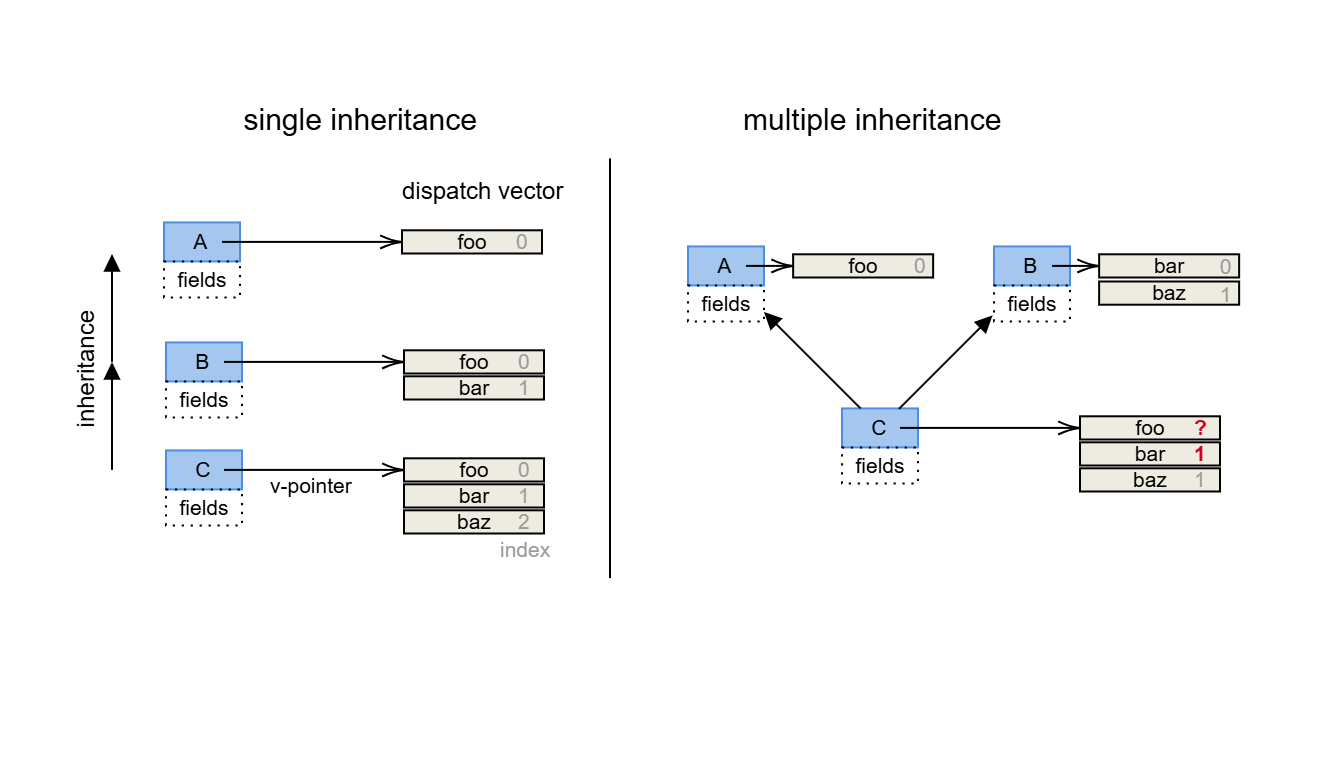
\includegraphics[width=1\linewidth]{images/inheritance.png}
\textbf{Solutions}
\begin{itemize}[leftmargin = *,noitemsep]
 \item One DV per superclass, calls use the dispatch vector corresponding to the static type at the call site. \textbf{Pros:} O(1), supports separate comp. \textbf{Cons:} Implicit casting, diamond inheritance doesn't work, \textbf{Procedure}: eval object, (\texttt{new C()}), get static type (\texttt{A x = new C()}), use v-ptr for type (\texttt{A}), used in c++
 \item Store class info structure, with pointer to superclass, mapping method-name to function pointer \textbf{Pros}: Caches optimize repeated calls to amortized O(1). Avoids index conflicts and supports multiple inheritance, \textbf{Cons}: Complex impl. \textbf{Procedure}: Look for f-name in class structure, if not found, move to superclass
 \item Every method is given global unique slot by compiler building inheritance graph, \textbf{Pros}: Fastest option, simple at runtime, \textbf{Cons}: No separate compl. possible, all code needs to be recompiled, different variants: Sparse DV Tables, Bin. Search Tree
 
 
 
 Compiler computes global method layouts using knowledge of the entire class hierarchy.
Each method gets a unique global slot; dispatch vectors may be sparse or replaced by decision structures. Enables fast dispatch with a single vptr, but breaks separate compilation and requires whole-program knowledge.
\end{itemize}


\mysection[black]{5. Optimisation \& Register Alloc.}

\mysubsection{5.1 Optimisation}
\textbf{90/10-Rule}: 90\% of the ex. time is spent in 10\% of the code, mostly loops\\
\textbf{Constant Folding}: If operands are statically known, compute val. and math. simplify: {\scriptsize \texttt{x = (2+3)*y} $\rightarrow$ \texttt{x = 5*y}}\\
\textbf{Const. Prop.}: Prop. var. if c.: {\scriptsize \texttt{x = 5; y = 2*x} $\rightarrow$ \texttt{y = 5*2}}\\
\textbf{Dead Code Elimination (DCE)}: Rem. side-effect free code:  {\scriptsize \texttt{x = y*y; x = z*z} $\rightarrow$ \texttt{x = z*z}} \\
\textbf{Common Subexpression Elimination (CSE)}: Fold redundant comp.:{\scriptsize \texttt{a[i] = a[i] + 1} $\rightarrow$ \texttt{[a + i*4] = [a + i*4] + 1}} \\
\textbf{Strength Reduction}: Replace exp. ops. with cheap ones  {\scriptsize \texttt{loop(a[i*3]=1; ...)} $\rightarrow$ \texttt{i=0; loop(a[i]=1; i=i+3; ...)}}\\
\textbf{Loop Invariant Code Motion (LICM)}: If res. of a expr. doesn't change in loop and it’s pure, can be moved outside body: {\scriptsize \texttt{loop(t=a.length; ...)} $\rightarrow$ \texttt{t=a.length; loop(...)}} \\
\textbf{Loop Unrolling}: Avoid cond. branches:{\scriptsize \texttt{for (int i=0; i<n; i++) \{ S \}} $\rightarrow$ \texttt{i;for (i=0; i<n-3; i+=4) \{S;S;S;S\};for ( ; i<n; i++) \{ S \}}}, unrolling $k$ el. $\frac{k}{k-1}$ branches \\
\textbf{Inlining}: Replace a function call with the body of the function with arguments rewritten to be local variables: pot. renaming var. to avoid naming capture\\
\textbf{Code Specialization}: Create specialized vers. of a fun. that is called from
diff. places with diff. args.\\
\textbf{Speedup[\%]}: $=\left[\frac{\operatorname{base time}}{\operatorname{opt. time}}-1\right]\cdot 100 \%$   



\mysubsection{5.2 Register Allocation}


\textbf{Register Allocation}: Place vars. in same registers if not alive at same time. Reg. much faster than mem.\\
\textbf{Liveness}: \texttt{X} live at \texttt{L} if def. before and used after\\
\textbf{Scoping}: Vars. in diff. scopes are cannot be alive simult.\\
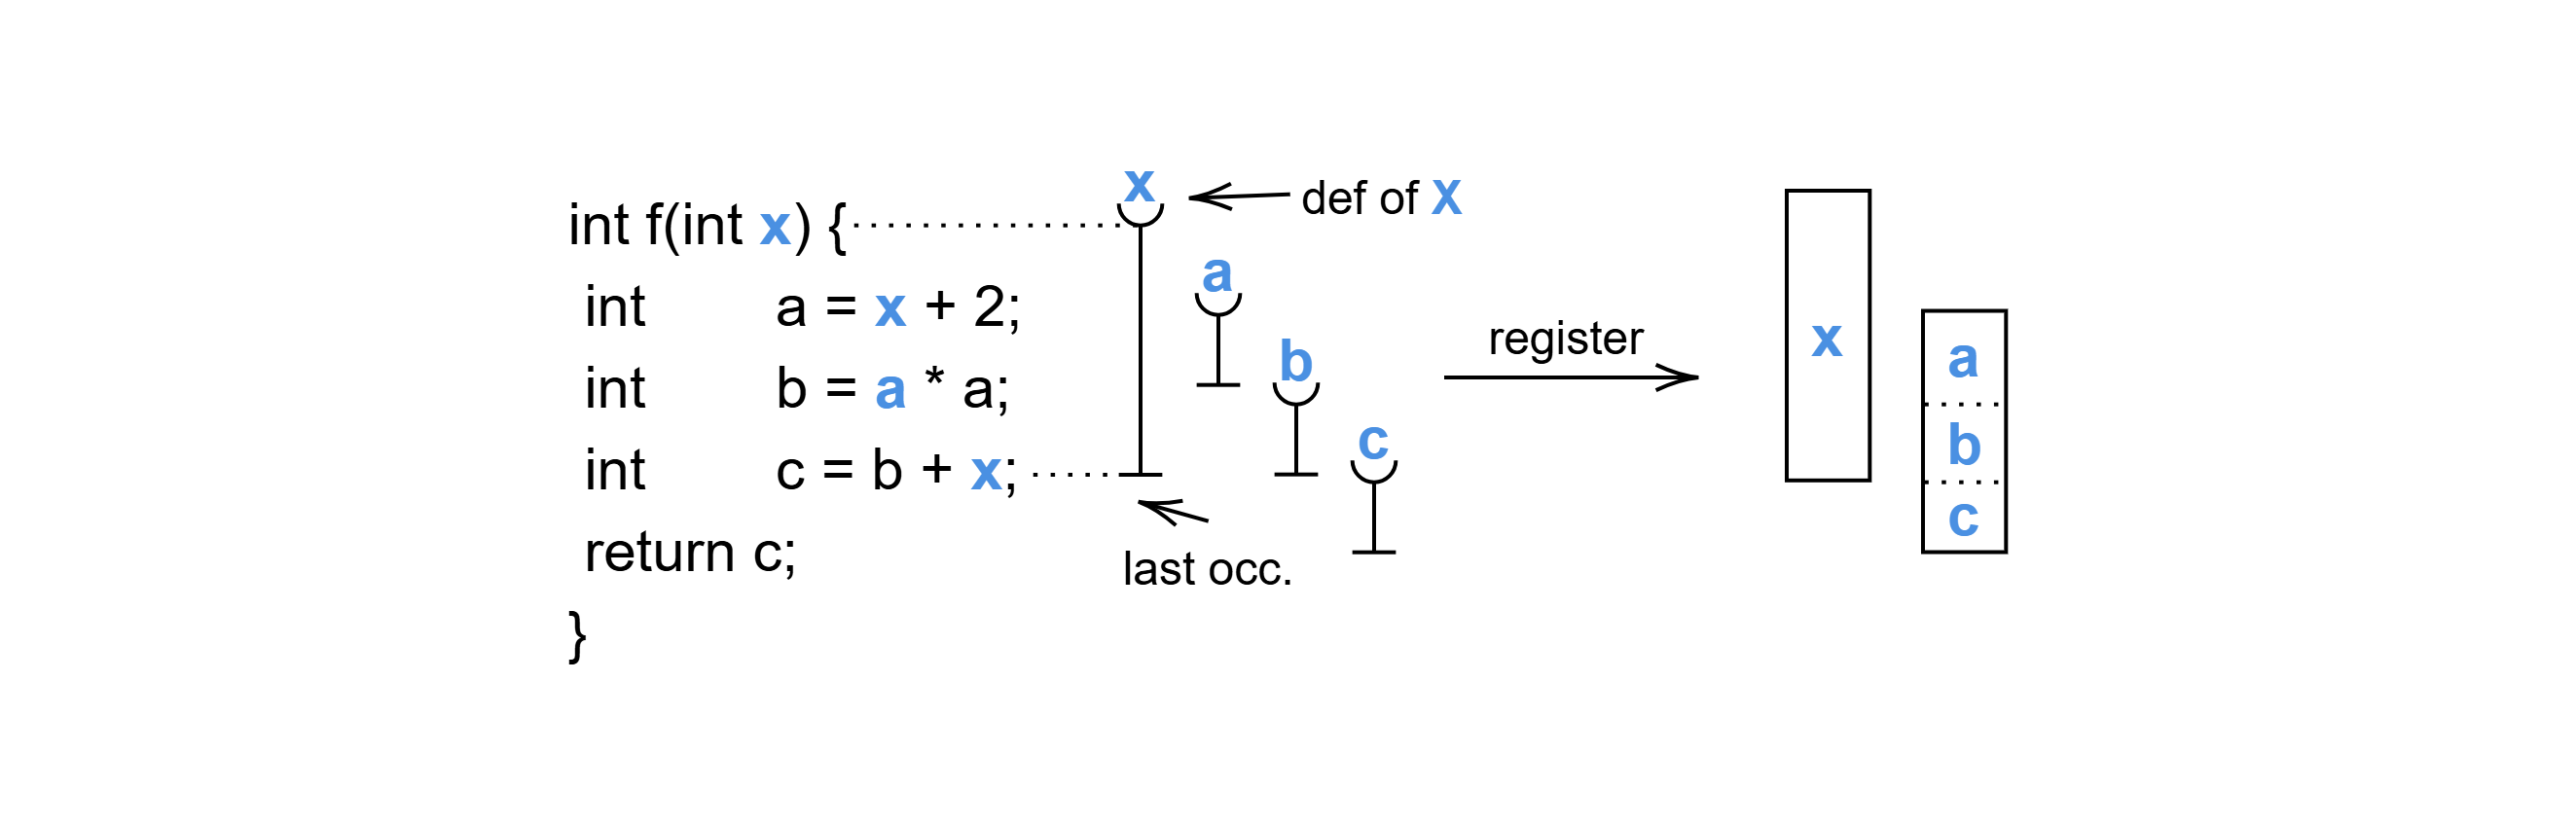
\includegraphics[width=1\linewidth]{images/liveness.png}
\textbf{Alloca Promotion}: Promote stack-allocated variables to SSA registers. Replace alloca + load/store with SSA values and ntroduce $\phi$-nodes where needed\\
\textbf{Stack Spilling}: If not all temps fit into register, spill excess to stack\\
\textbf{Linear-Scan Register Allocation}: 1. Compute set of uids: $\operatorname{live}(x)$ 2. def $\operatorname{pal}$ as usable registers 3. maintain layout by $\operatorname{uid\_loc}$ 4. For each instr. that defines uid $x$: $\operatorname{used} =  \left\{ r \mid \operatorname{reg} r =  \operatorname{uid\_loc}(y) \text{ s.t. } y \in \operatorname{live}(x)\right\}$, $\operatorname{available}= \operatorname{pal} - \operatorname{used}$, if $\operatorname{available}= \emptyset$  then $\operatorname{uid\_loc}= \operatorname{slot}n; n++$ else   $\operatorname{uid\_loc}=\operatorname{reg} r \in \operatorname{available}$, Note that any vars. live over multiple loop iterations are allocated first
\\

\textbf{Graph Coloring}: Compute liveness info for each temp, create interference graph i.e. $E(b_1,b_2)$ iff both are live simult., color graph
\mysection[black]{6. Flow \& GC}


\mysubsection{6.1 Control Flow}
\textbf{Block}: Single entry point, seq. of (possibly empty) instr, ends with single control-flow instr.\\
\textbf{Control-Flow Graph (CFG)}: Nodes are blocks, $E(b_1,b_2)$ iff $b_1$ may jump to $b_2$\\
\textbf{Domination}: $A$ dominates $B$: if the only way to reach $B$ from start node is via $A$\\
\textbf{Back Edge}: Edge in CFG where target dom the source $E(n,h) \wedge n \in \operatorname{dom}[h]$, $h$=header, \textcolor{red}{be aware: transitive !} \\
\textbf{Natural Loop (NL)}: Given back edge $E(n,h)$, NL is set of nodes dominated by $h$, that can reach (in CFG) $n$ without passing through $h$ $\cap \{h\}$ \\
\textbf{Dominator Dataflow Analysis (DDA)}: Computed using a forward, must dataflow anal.\\
\textbf{Algorithm for DOM-Trees}: 
\begin{enumerate}[leftmargin = *,noitemsep]
\item  Init $\operatorname{dom}[\operatorname{entry}]=\{\operatorname{entry}\}$,$\operatorname{dom}[n]=\{\forall n \in \operatorname{CFG}\}$
\item Iter. until conv. $\operatorname{dom}[n] = \{n\}\cup \bigcap_{p\in \operatorname{pred}[n]}\operatorname{dom}[p]$
 \end{enumerate}
\textbf{Dom-Trees (DT)}: All CFG have DT, built through DDA, properties: transitive $A  \operatorname{dom} B \vee B  \operatorname{dom} C\Rightarrow A  \operatorname{dom} C$, anti-symmetric $A  \operatorname{dom} B \vee B  \operatorname{dom} A\Rightarrow A = B$\\
\textbf{Dominance Frontier (DF)}: of a node $B$ is the set of all CFG nodes $y$ such
that $B$ dominates a predecessor of $y$, but does not strictly dominate $y$\\
\textbf{Algo (from CFG)}: $\forall n: \forall p \in \operatorname{pred}[n] \left(\right.r = p;$ $ \operatorname{while}(r \neq \operatorname{doms}[B])\left\{ \operatorname{DF}[r]:= \operatorname{DF}[r] \cup B; r:= \operatorname{DF}[r]\right\}\left.\right)$\\
\textbf{Algo (from DF)}: Given nodes $N$, compute $\operatorname{DF}[S]=\bigcup_{n \in N} \operatorname{DF}[n]$ Repeat until convergence: $S \leftarrow S \cup \operatorname{DF}(S)$\\

\mysubsection{6.2 Data Flow (DF)}
\textbf{DF Anal.}: Compute liveness $\forall$ vars. simult.\\
\textbf{Use/Def}: $\operatorname{use}[s]$/$\operatorname{def}[s]$ set of var. used/defined by $s$\\
\textbf{In/Out}: $\operatorname{in}[n]$/$\operatorname{out}[n]$ set of var. live on entry/exit of $n$\\
\textbf{Gen/Kill}: $\operatorname{gen}[n]$/$\operatorname{kill}[n]$: info. generated/invalidated by $n$ \\


\textbf{Liveness}: Variable $v$ is live on edge $e$ if:
\begin{enumerate} [leftmargin = *,noitemsep]
\item a node $n$ in the CFG such that $v\in \operatorname{use}[n]$, and
\item a dir. path $P(e,n)$ s.t $\forall s' \in P(e,n)\Rightarrow v \not \in \operatorname{def}[s']$
\end{enumerate}
\textbf{Computational Inference Conditions}:

\begin{multicols}{2}
\begin{center}
    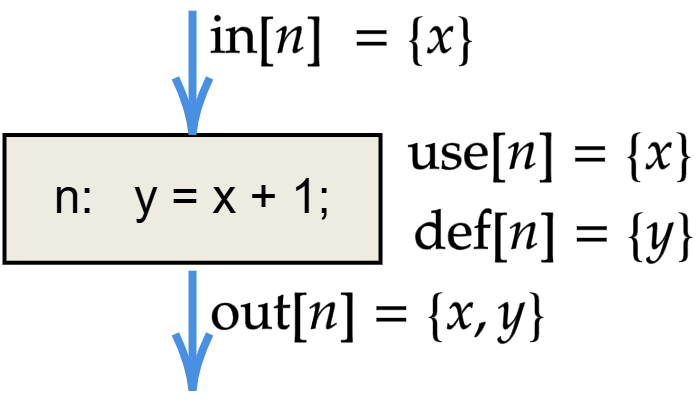
\includegraphics[width=0.75\linewidth]{images/defs.png}
\end{center}
\columnbreak
\begin{enumerate} [leftmargin = *,noitemsep]
\item $\operatorname{in}[n] \supseteq \operatorname{use}[n]$
\item $\operatorname{in}[n] \supseteq \operatorname{out}[n]\operatorname{def}[n]$
\item $\operatorname{out}[n] \supseteq  \operatorname{in}[n'] \text{ if } n' \in\operatorname{succ}[n]$
\end{enumerate}
\end{multicols}

\textbf{Iter. Anal}: Start with $\operatorname{in}[n]=\operatorname{out}[n]=\emptyset$ and converge\\
\textbf{Algo}: Set $\forall n.\operatorname{in}[n]=\operatorname{out}[n]=\emptyset$. Repeat until guaranteed convergence i.e. no change in $\operatorname{in}$ and $\operatorname{out}$: {\footnotesize $\forall n. \left[ \operatorname{out}[n]=\bigcup_{n'\in \operatorname{succ}[m]}\operatorname{in}[n']\text{ then} \operatorname{in}[n]= \operatorname{use}[n] \cup \left(\operatorname{out}[n] \setminus \operatorname{def}[n]\right) \right]$ }\\

\textbf{Meet-Over-Path (MOP)}: Solution that accounts for all possible paths in the CFG: $\bigcap_{p \in \operatorname{paths_to}[n]}\ell_p$, where $\ell_p$ is dataflow info (liveness ...)\\
\textbf{Iter. Sol.}: Converges to MOP sol, if distributive $\bigcap_i F_n (\ell_i)= F_n (\bigcap_i \ell_i)$\\
\textbf{Distributive properties}: Program structure: liveness, available expr, reaching def, busy expr\\
\textbf{Non-Distr. prop.}: What is computed: output = pos. ?, constprop\\



\begin{center}
\begin{tabular}{lll}
\hline
\textbf{Analysis} & \textbf{Type} & \textbf{Equations} \\
\hline

Liveness &
BW, May &
{\tiny $
\begin{array}{l}
\text{out}[n] := \bigcup_{n' \in \mathrm{succ}[n]} \text{in}[n'] \\
\text{in}[n] := \text{use}[n] \cup (\text{out}[n] \setminus \text{def}[n])
\end{array}$}
\\[1.5ex]

Reaching Def. &
FW, May &
{\tiny $
\begin{array}{l}
\text{in}[n] := \bigcup_{p \in \mathrm{pred}[n]} \text{out}[p] \\

\end{array}$}
\\[1.5ex]

Available Expr. &
FW, Must &
{\tiny $
\begin{array}{l}
\text{in}[n] := \bigcap_{p \in \mathrm{pred}[n]} \text{out}[p] \\
\text{out}[n] := \text{gen}[n] \cup (\text{in}[n] \setminus \text{kill}[n])
\end{array}$}
\\[1.5ex]

Constant Prop. &
FW, May &
{\tiny $
\begin{array}{l}
\text{in}[n] := \bigcup_{p \in \mathrm{pred}[n]} \text{out}[p] \\
\text{out}[n] := \text{transfer}_n(\text{in}[n])
\end{array}$}
\\[1.5ex]

Alias Anal. &
FW, May &
{\tiny $
\begin{array}{l}
\text{in}[n] := \bigcup_{p \in \mathrm{pred}[n]} \text{out}[p] \\
\text{out}[n] := \text{transfer}_n(\text{in}[n])
\end{array}$}
\\

Busy Expr. &
BW, Must&
{\tiny $
\begin{array}{l}
\text{out}[n] := \bigcap_{p \in \mathrm{succ}[n]} \text{in}[p] \\
\text{in}[n] := \operatorname{gen}[n] \cup \left(\operatorname{out}[n] \setminus \operatorname{kill}[n]\right)
\end{array}$}
\\
\hline
\end{tabular}
\end{center}






\mysubsection{6.3 GC}
\textbf{Reachability}: $X$ is reachable iff A register contains a pointer to $X$, or another reachable object contains a pointer to $X$, approximation if object is used or not\\
\textbf{GC Scheme}: 1. Allocate space for new ojects, 2. Compute objects that might be used again, free space not in the found objects from before\\

\textbf{Mark and Sweep}: Each Object has mark bit ($1\Leftrightarrow$ reachable); When memory runs out, GC does: 1. Mark Phase: Trace reachable objects 2. Sweep Phase: Collect garbage object, add to free list, fragmentation possible\\
\textbf{Pointer Reversal}: Stackless graph traversal, temporarily reversing heap ptr, s.t. store the parent, when traversing back original pointer is restored\\
\textbf{Stop and Copy}: Mem. org. in 2 areas: Old- (OS) \& new Space (NS), Heap pointer points to next free word in OS. When OS is full: 1. Copy reachable objects into NS 2. Reverse role of NS and OS. , Generally fastest method, cannot be done in C, as copying is impossible\\
\begin{center}
    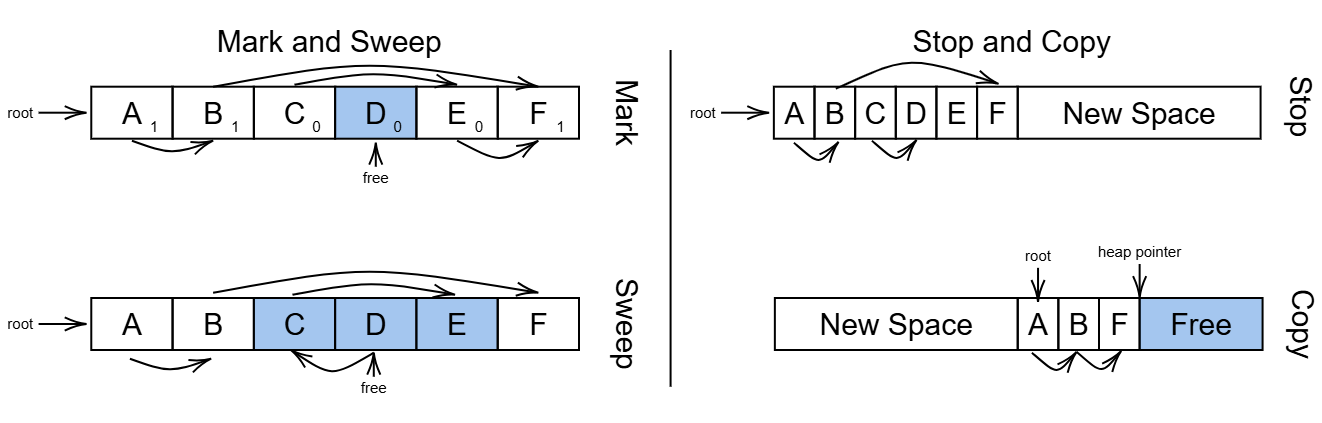
\includegraphics[width=1\linewidth]{images/gc.png}
\end{center}
\textbf{Reference Counting}: Keeps track of number of ptr to object, very slow, not possible for circular structures \\



\mysection[black]{6. MC}


\scriptsize
\hspace{3mm}



{\normalsize\textbf{x86/LLVM}}

\textbf{Which of the following statements are correct about x86?}
\begin{itemize}

\item[\textcolor{red}{W}] Every x86 instruction pushes its result onto the stack.
\item[\textcolor{green}{C}] The operand of an x86 instruction can be a register, a machine address, a literal,or a label.
\item[\textcolor{red}{W}] x86 instructions store intermediate results into the heap.
\item[\textcolor{red}{W}] x86 instructions can only access the heap via the stack.
\end{itemize}


\textbf{Which of the following statements is wrong about the X86-64 System V ABI calling convention?}
\begin{itemize}

\item[\textcolor{green}{C}] Integer return values of functions are stored into the \%rax register
\item[\textcolor{red}{W}] The callee sets up its stack frame by updating the location where \%rsp and \%rbp point to.
\item[\textcolor{green}{C}] Every argument of a callee function is stored into registers by the caller
\item[\textcolor{green}{C}] The callee function is responsible for destroying its stack frame
\end{itemize}



\textbf{What’s the semantics of movq (\%rsi), \%rdi in x86?}
\begin{itemize}
\item[\textcolor{green}{C}] Interprets the contents of \%rsi as an address, and then copies the contents ofthis address to register \%rdi. 

\end{itemize}



\textbf{What is/are the purpose(s) of using LLVM IR in a compiler middle-end ratherthan x86 assembly or C code?}
\begin{itemize}

\item[\textcolor{green}{C}] Multiple compiler back-ends (x86, ARM, RISC-V, etc) can use the same compilermiddle-end.
\item[\textcolor{red}{W}] LLVM IR does not encode control-flow information
\item[\textcolor{green}{C}] Multiple compiler front-ends (source languages) can use the same middle-end.
\item[\textcolor{green}{C}] Assembly or C code are more difficult to analyze and optimize.
\end{itemize}


\textbf{Which of the following statement(s) is/are correct about LLVM IR?}
\begin{itemize}
\item[\textcolor{red}{W}] Instructions are not typed.
\item[\textcolor{red}{W}] Basic blocks can contain multiple control-flow instructions.
\item[\textcolor{green}{C}] Only the last instruction of a basic block is called the terminator.
\item[\textcolor{green}{C}] Local variables must satisfy the single static assignment invariant.
\end{itemize}


\textbf{Which of the following statement(s) is/are correct about the control-flow graph in LLVM IR?}
\begin{itemize}

\item[\textcolor{green}{C}] Nodes are basic blocks, and basic blocks contain instructions.
\item[\textcolor{green}{C}] An edge in control-flow graph represents a conditional/unconditional jump froma source block to a target block.
\item[\textcolor{green}{C}] Basic blocks contain no interior label used as a jump target.
\item[\textcolor{green}{C}] Basic blocks must end with a control-flow instruction.
\end{itemize}



\textbf{Which of the following statement(s) is/are correct about manipulating pointersin LLVM IR}
\begin{itemize}

\item[\textcolor{green}{C}] \texttt{getelementptr} does not access memory.
\item[\textcolor{red}{W}] \texttt{getelementptr} traverses the links of a data structure to find the target object.
\item[\textcolor{red}{W}] \texttt{getelementptr} uses only constant indices to compute offsets.
\item[\textcolor{green}{C}] Returning a big (more than 64 bytes) structure object from a function can beachieved by passing a pointer argument allocated by the caller.
\end{itemize}



\textbf{Which of the following statement(s) is/are correct about manipulating pointersin LLVM IR}
\begin{itemize}
\item[\textcolor{green}{C}] Arguments \& return values are handled according to the calling conventions
\item[\textcolor{green}{C}] \texttt{getelementptr} is transformed into the form of base address + offset
\item[\textcolor{red}{W}] Array access indices are computed at compile time.
\item[\textcolor{green}{C}] Basic blocks are connected via conditional, unconditional, and implicit (fallthrough) jumps.
\end{itemize}



\textbf{Which of the following optimization(s) can be done at the LLVM-IR level?}
\begin{itemize}

\item[\textcolor{green}{C}]  Constant propagation
\item[\textcolor{red}{W}]  Dead code elimination
\item[\textcolor{green}{C}] Branch prediction
\item[\textcolor{green}{C}]  Value numbering
\end{itemize}







\end{flushleft}
\end{multicols}

\newpage





\end{document}

